%this file shows the Latex rules
%a % comment anything after % until the end of the line

%minimum references to begin our article
\documentclass[12pt]{article}
\usepackage[english]{babel}
\usepackage[utf8]{inputenc}
\usepackage[T1]{fontenc}
\usepackage{graphicx}
% the last extension makes it possible to add images

%la bibliographie ne fonctionne pas
\bibliographystyle{plain}
\bibliography{bibliography}

%presentation of the document
%title, author, date, thanks (optional)
\title{\LaTeX First try}
\author{Dan\thanks{Thanks to slides Internet and Benoit}}
\date{08/10/2014}
\begin{document}
\maketitle
\begin{abstract}
This is the text of my abstract :
Lorem ipsum dolor sit amet, consectetur adipiscing elit. Ut eu est laoreet, egestas ipsum id, cursus metus. In ut fringilla massa. In hac habitasse platea dictumst. In laoreet, ex id scelerisque rhoncus, purus mauris fermentum metus, vel egestas lacus nunc quis massa. Aenean efficitur volutpat risus. Vivamus ultrices mi ac nisl elementum, in placerat quam pellentesque. Integer suscipit, elit a egestas luctus, leo libero efficitur diam, sit amet porttitor mi nibh pellentesque metus. Fusce ultrices, ligula quis lacinia rutrum, sem enim laoreet dui, et auctor lectus ligula vel augue.\newline
This is the end of my abstract
\end{abstract}
% to create an abstract, just use begin and end with abstract

Enter Text here

\newpage
%to add a table of contents
\tableofcontents
\newpage

%to create sections and subsections, we can use : (chapter n'existe pas avec la classe article)
\part{part 1 : how to do this}
\section{Section}
\subsection{Subsection}
\paragraph{Paragraph title}

My paragraph : Lorem ipsum dolor sit amet, consectetur\footnote{I am a footnote and I know it} adipiscing elit. Ut eu est laoreet, egestas ipsum id, cursus metus. In ut fringilla massa. In hac habitasse platea dictumst. In laoreet, ex id scelerisque\underline{ rhoncus, purus} mauris \textit{fermentum metus nunc quis massa}. Aenean efficitur volutpat risus. \textbf{Vivamus ultrices mi ac nisl elementum}, in placerat quam pellentesque. Integer suscipit, elit a egestas lu  \cite{cc} 
%bold and italic are handled by textit and textbf, underlined with underline
%to use a footer, use footnote{I am a foot note}

%adding images using includegraphics[scale][path]
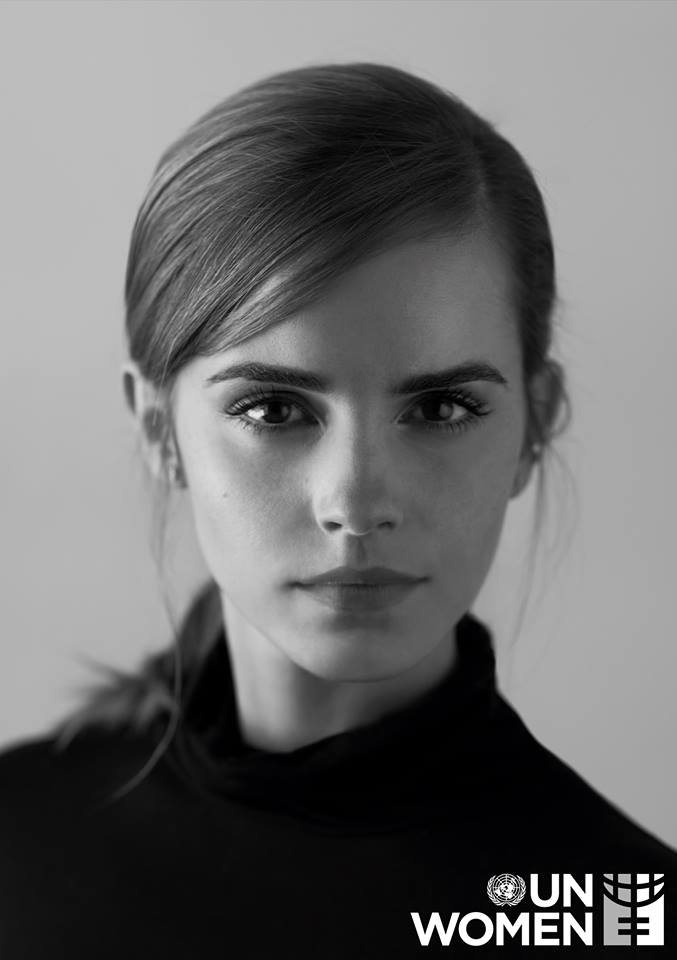
\includegraphics[scale=0.2]{picture}

\includegraphics[scale = 0.2]{img/picture2}
\newpage

%adding image with caption begin(name)[position h t top b bottom p flottant], centerline for putting in the center
\begin{figure}[t]
\centerline{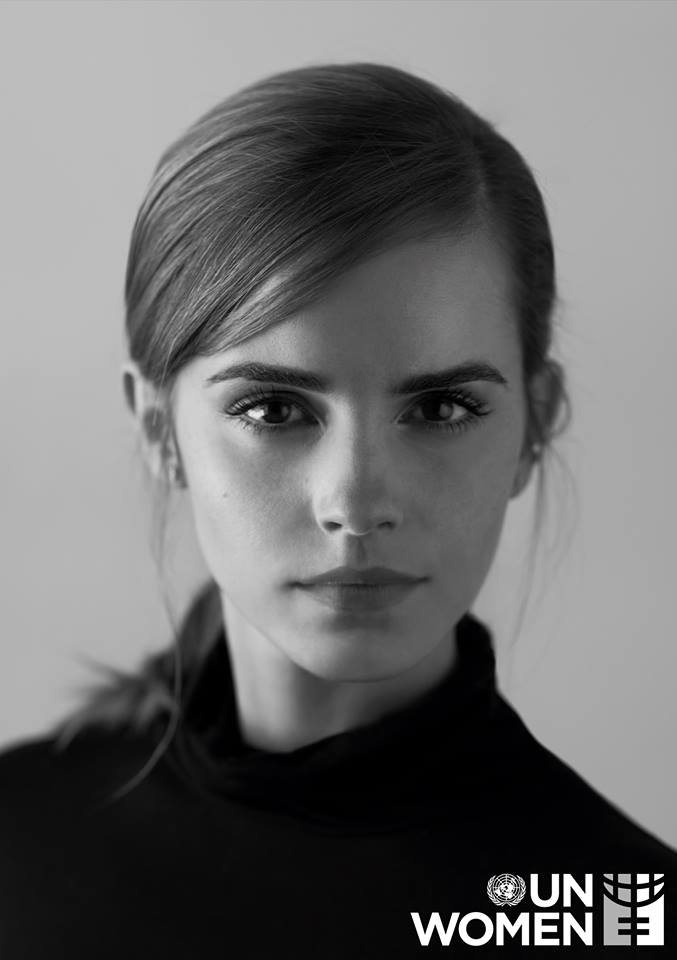
\includegraphics[scale=0.35]{picture}}
   \caption{\label{étiquette} this is emma watson}
\end{figure}
\newpage


%to make a numerized list, we have to use \begin{enumerate} \item then and finally \end{enumerate}
We are going to attend this conferences :
\begin{enumerate}
\item James Bond car
\item Medical applications for tomorrow
\item How to be an entrepreneur at the INSA de Rennes
\end{enumerate}

\bigbreak
\bigbreak

%to make a list of item \begin{itemize} then \item nameItem finally \end{item}
Items :
\begin{itemize}
\item Carrots
\item Potatoes
\end{itemize}

\bigbreak
\bigbreak

%to jump a line in this file won't work in the final file, we need to use : \smallbreak or \medbreak or \bigbreak
How to jump a line ?

Jump line smallbreak
\smallbreak
Jump line medbreak
\medbreak
Jump line bigbreak
\bigbreak
I suggest mediumlbreak

%How to end a line newline or linebreak with text ordered
I want to end the line \newline
I Want to end the line on a better way (justifié) \linebreak

\bigbreak
\bigbreak

%how to make a table tabular
% to begin \begin{tablular}, finally \end{tabular} 
% to change lines on the table : change |l|c|r|
%to separate elements in a table, use &
% to end a line \\
% to jump a line for the next one \hline (on one line just \\ \hline)
%to separate lines, 
\begin{tabular}{|l|c|r|}
  \hline
  Column 1 & Column 2 & Column 3 \\
  \hline
  Line1 & 1.2 & 1.3 \\  \hline
  Line2 & 2.2 and his friend are in a boat& 2.3 \\ \hline
\end{tabular}



%how to jump a page : newpage or pagebreak if ordered text
\newpage

Next page with a newpage
\end{document}
%end marker of the document
